\documentclass[11pt]{article}

\usepackage[margin=1in]{geometry}
\usepackage{graphicx}
\usepackage{amsmath}
\usepackage{amssymb}
\usepackage{booktabs}
\usepackage{hyperref}
\usepackage{listings}
\usepackage{xcolor}
\usepackage{caption}
\usepackage{parskip}

\hypersetup{
  colorlinks=true,
  linkcolor=blue!50!black,
  citecolor=blue!50!black,
  urlcolor=blue!50!black
}

\definecolor{listingbg}{rgb}{0.97,0.97,0.97}
\definecolor{listingrule}{rgb}{0.80,0.80,0.80}

\lstdefinestyle{cstyle}{
  language=C,
  basicstyle=\ttfamily\small,
  keywordstyle=\color{blue!60!black}\bfseries,
  commentstyle=\color{gray!60!black}\itshape,
  stringstyle=\color{red!50!black},
  backgroundcolor=\color{listingbg},
  frame=single,
  framerule=0.4pt,
  rulecolor=\color{listingrule},
  numbers=none,
  showstringspaces=false,
  breaklines=true,
  captionpos=b,
  xleftmargin=0.6em,
  xrightmargin=0.4em,
  belowskip=0.6em
}

\lstdefinestyle{pseudostyle}{
  basicstyle=\ttfamily\small,
  backgroundcolor=\color{listingbg},
  frame=single,
  framerule=0.4pt,
  rulecolor=\color{listingrule},
  numbers=none,
  showstringspaces=false,
  breaklines=true,
  captionpos=b,
  xleftmargin=0.6em,
  xrightmargin=0.4em,
  belowskip=0.6em,
  morekeywords={if,else,for,while,return,end,foreach,select,procedure,function,then,do},
  keywordstyle=\color{blue!60!black}\bfseries,
  commentstyle=\color{gray!60!black}\itshape
}

\title{Online Behavioral Scheduling in a From-Scratch RISC-V Kernel}
\author{Ayan Goel}
\date{}

\begin{document}
\maketitle

\begin{abstract}
Production schedulers like Linux CFS and classical multi-level feedback
queues run on heuristics that were tuned decades ago. This project builds a
RISC-V 64-bit kernel from bare metal and layers five hot-swappable scheduling
policies on top: round-robin, MLFQ, and three online-learning variants. They
get measured on a matrix of eight workloads, two of them adversarial. The
strongest learning policy, an online behavioral classifier with windowed
inputs, beats MLFQ on every workload in the matrix and matches its
phase-change adaptation speed. A more ambitious contextual-bandit scheduler
loses on cpu-heavy workloads because UCB exploration eats the test budget.
The interesting result isn't a new algorithm. It's that, on this kernel and
these workloads, simple online statistics outperform both fixed heuristics
and gradient-based bandits.
\end{abstract}

\section{Motivation}
\label{sec:motivation}

Production schedulers carry a lot of decades-old policy. CFS replaced the
O(1) scheduler in Linux 2.6.23~\cite{cfs}; MLFQ traces back to the early
1960s. The heuristics they encode (priority decay, quantum doubling, virtual
runtime) were tuned for workloads that look very little like what modern
processes actually do. So: can a scheduler that watches what each process
does and updates its policy online make better decisions than one operating
from a fixed rulebook?

That question is hard to answer in a Linux fork. The kernel is too large to
hold in your head, the trace surface is too noisy, and any policy change
competes with thousands of unrelated decisions the kernel is making at the
same time. The way out is to build a smaller kernel. Small enough that every
scheduling decision and every byte of per-process state is visible and
modifiable; large enough to run a realistic mix of CPU-bound, I/O-bound, and
adversarial workloads. That is the kernel this project builds.

\section{The Kernel}
\label{sec:kernel}

The kernel is RISC-V 64-bit (\texttt{rv64gc}), about 3{,}500 lines of C plus
a small amount of assembly for the entry stub, trap vector, and context
switch. It runs on QEMU's \texttt{virt} machine and sits entirely in machine
mode~\cite{riscvspec}, dropping into user mode via \texttt{mret}.

The pieces:

\begin{itemize}
  \item \textbf{Trap path.} \texttt{mtvec} points at a hand-written vector
  that saves 31 GPRs into a trap frame and dispatches on \texttt{mcause}.
  \texttt{mscratch} holds the kernel stack pointer when user code is running
  and zero when kernel code is, so trap entry can swap stacks atomically with
  a single \texttt{csrrw}.

  \item \textbf{Paging.} Sv39, with kernel mappings shared across processes
  and user mappings carved into a single root-table slot. \texttt{vm\_check\_wx}
  runs at boot and panics if any kernel page is mapped both writable and
  executable.

  \item \textbf{Processes.} A 64-slot process table; each slot owns a 4\,KB
  kernel stack, a per-process page table, a saved context, and a trap frame.
  Lifecycle: \texttt{UNUSED} $\to$ \texttt{EMBRYO} $\to$ \texttt{RUNNABLE}
  $\to$ \texttt{RUNNING} $\to$ \texttt{SLEEPING} or \texttt{ZOMBIE} $\to$
  \texttt{UNUSED}. Syscalls implemented: \texttt{fork}, \texttt{exec},
  \texttt{wait}, \texttt{exit}, \texttt{write}, \texttt{getpid},
  \texttt{yield}, \texttt{sleep}.

  \item \textbf{Shell and TUI.} An ANSI-rendered dashboard runs as a kernel
  thread, redrawing at roughly 20\,fps over the UART. A shell command parses
  input from the same UART. \texttt{sched <name>} hot-swaps the active
  scheduler with no reboot; \texttt{run <prog>} forks and execs a workload;
  \texttt{trace 200} dumps the last 200 scheduler events as ASCII.

  \item \textbf{Trace ring.} Every scheduling-relevant transition (RUN,
  YIELD, PREEMPT, SLEEP, WAKE, SPAWN, EXIT, DEMOTE, BOOST) writes one 8-byte
  record into a 16K-entry static ring. The shell dumps it on demand. The
  Python parser in \texttt{tools/parse\_trace.py} turns the dump into CSVs
  and matplotlib Gantt charts.
\end{itemize}

Two constraints apply throughout. No floating point anywhere in the kernel,
so every scheduler statistic is fixed-point integer math. No allocation in
the scheduling hot path. The scheduling code can read and update fields on
\texttt{proc\_t} but cannot call into \texttt{kmalloc}.

The point of the kernel isn't the kernel. It's a measurement surface for
comparing scheduling policies on identical hardware with identical
workloads.

\section{Scheduler Design}
\label{sec:design}

Every policy implements the same five-callback interface:

\begin{lstlisting}[style=cstyle]
typedef struct sched_policy {
    const char  *name;
    struct proc *(*pick_next)(void);
    void  (*on_burst_end)(struct proc *p);
    int   (*should_preempt)(struct proc *p);
    void  (*on_periodic)(void);
    void  (*on_proc_init)(struct proc *p);
    void  (*on_activate)(void);
} sched_policy_t;
\end{lstlisting}

\texttt{pick\_next} returns the next runnable process to dispatch.
\texttt{on\_burst\_end} fires when the running process yields, sleeps, is
preempted, or exits. \texttt{should\_preempt} is called from the timer ISR
and decides whether to call \texttt{sched()} now or let the burst continue.
The other callbacks are policy bookkeeping. Adding a new policy is roughly
``fill in these five.''

\subsection*{RR --- Round-robin}

Cursor sweep over \texttt{proc\_table}; one RUNNABLE slot per call;
\texttt{should\_preempt} always returns 1. Per-process state: none. Cost per
decision: at most 64 slot reads.

\subsection*{MLFQ --- Multi-level feedback queue}

Four priority levels with allotments \{1, 2, 4, 8\} ticks. Quantum-expiry
preempts demote one level; voluntary yields keep the current level; a
periodic boost every 100 ticks promotes everyone back to level 0. Standard
OSTEP MLFQ~\cite{ostep}. Per-process state: \texttt{mlfq\_level} (1 byte),
\texttt{mlfq\_used\_in\_level} (2 bytes), \texttt{mlfq\_demote\_count}
(8 bytes for stats).

\subsection*{V1 --- Exponentially-weighted burst predictor}

For each process keep an estimate $\tau$ of its recent burst length and pick
the runnable process with the smallest $\tau$ (approximate SRTF). Update on
each burst close:
\[
\tau_{n+1} = \frac{1}{2} \cdot t_n + \frac{1}{2} \cdot \tau_n
           = (t_n + \tau_n) \gg 1
\]
Stored at 8$\times$ scale (three fractional bits) so 1-tick bursts converge
to a stable non-zero value rather than collapsing to 0 under the integer
right-shift. Per-process state: \texttt{burst\_estimate} (4 bytes). Cost per
decision: one linear scan with min tracking.

\subsection*{V2 --- Online classifier + per-class quantum}

V2 classifies each process into one of four behavioral classes and assigns a
class-specific quantum. The classifier is a hand-coded threshold tree, not a
learned model:

\begin{lstlisting}[style=pseudostyle]
function v2_classify(proc):
  sl, yi, pr = recent-window counts of {sleep, yield, preempt}
  if yi > sl and yi > pr and burst_estimate <= 8:
      return INTERACTIVE        # 1-tick quantum
  if sl > pr:
      return IO_BOUND           # 1-tick quantum
  if pr > 0 and pr >= sl:
      return CPU_BOUND          # 5-tick quantum
  return BATCH                  # 10-tick quantum
\end{lstlisting}

The classifier is re-run on every burst end. \texttt{pick\_next} scans by
class in priority order (INTERACTIVE first, BATCH last); within each class
it round-robins. Kernel threads are pinned to BATCH at pick time regardless
of their stored class. Per-process state: 22 bytes for the windowed
classifier (Section~\ref{sec:phase7} describes the windowed counters
specifically).

\subsection*{V3 --- Contextual bandit}

V3 treats each scheduling decision as a bandit problem. For each runnable
process, compute an 8-feature context vector
$\mathbf{x} = (\tau, \sigma^2, \text{yield\_ratio}, \text{io\_rate},
t_{\text{since\_run}}, \text{class}, \text{age}, 0)$
and score with a learned linear value function
$V(\mathbf{x}) = \mathbf{w}^\top \mathbf{x} + c \cdot (1/(n_i + 1))$,
where the second term is a UCB exploration bonus over visit counts $n_i$.
On each burst close, update the weights with a gradient step:
\[
w_i \mathrel{+}= (r \cdot x_i) \gg 10, \quad
r = -t_n + \mathbb{1}[\text{state} = \text{SLEEPING}]
\]
All arithmetic is integer; weight updates are right-shifted by 10 (an
implicit learning rate of $1/1024$). Per-process state: 32 bytes for the
context plus a 4-byte visit count; one global 32-byte weight vector.

The spec said V3 should be $O(1)$ per decision via a sorted runnable list.
The implementation sweeps \texttt{proc\_table} once per decision instead, so
it is $O(\text{NPROC})$ with NPROC$=64$. The deviation is documented in the
source and revisited in Section~\ref{sec:future}.

\section{Methodology}
\label{sec:method}

\textbf{Workloads.} Eight synthetic user programs, all compiled with the
same toolchain and embedded in the kernel image. Six came from earlier
phases (\texttt{cpu\_bound}, \texttt{io\_bound}, \texttt{mixed},
\texttt{bursty}, \texttt{forker}, \texttt{concurrent}). Two adversarial
workloads were added for this phase. \texttt{flipper} runs 10 short sleeps
then 5 rounds of tight compute, forcing an I/O$\to$CPU phase change mid-run.
\texttt{wolf} runs 100 single-tick \texttt{sleep(1)} calls then 5 rounds of
compute, the classical MLFQ priority-gaming exploit.

Each workload is sized so the scheduler makes at least 100 decisions per
process at a 10\,ms quantum. Below that, per-decision overhead variance
drowns out the policy signal.

\textbf{Metrics.}
\begin{itemize}
  \item \textbf{events:} total trace records during the run window. A proxy
  for total scheduler decisions at fixed wall-clock. Lower is better.
  \item \textbf{preempts:} involuntary preemptions of the workload's
  primary pid.
  \item \textbf{run\_ticks:} sum of RUN-interval widths, in 10\,ms ticks.
  \item \textbf{cyc/dec:} mean CPU cycles per \texttt{pick\_next} call,
  captured by reading the \texttt{rdcycle} CSR immediately before and after
  the call site in \texttt{scheduler()}. Per-policy accumulators in
  \texttt{sched.c} sum cycles and decisions; a new \texttt{cycles} shell
  command dumps them at run end.
  \item \textbf{adaptation-speed} (\texttt{flipper} only): bursts after the
  I/O$\to$CPU phase change before the workload receives a burst
  $\geq 5$ ticks long. ``N/A'' for policies that don't adapt.
\end{itemize}

\textbf{Run protocol.} For each (policy, workload) cell:
boot the kernel, wait 8\,s for init's boot-time children to finish, set the
quantum to 10\,ms, hot-swap to the policy under test, clear the trace ring,
spawn the workload, wait 6\,s (12\,s for \texttt{flipper} and \texttt{wolf}
so both phases complete), dump the trace ring, dump the \texttt{cycles}
snapshot, exit QEMU. The full matrix is 5 policies $\times$ 8 workloads $=
40$ cells. \texttt{tools/run\_experiments.sh 6} runs it headlessly.

\textbf{Caveats.} QEMU TCG is not real hardware; cache behavior, branch
prediction, and ISR latency all differ from a real RISC-V CPU. The
tick-resolution timer is the floor for any burst-length statistic;
sub-tick discrimination would need \texttt{rdcycle}-based instrumentation on
the input side, which is left for future work.

\section{Results}
\label{sec:results}

\subsection*{The headline matrix}

Table~\ref{tab:headline} reports trace-record counts and workload-pid
preempts for each policy on each workload. Lower events is better (less
scheduler overhead at the same wall-clock). The V2 column is the Phase 7
windowed-classifier version; the Phase 6 V2 numbers are in
Section~\ref{sec:phase7}.

\begin{table}[h!]
\centering
\caption{Trace records / workload-pid preempts under each policy.}
\label{tab:headline}
\begin{tabular}{lrrrrr}
\toprule
workload    & RR        & MLFQ      & V1        & \textbf{V2 (P7)} & bandit  \\
\midrule
cpu\_bound  & 73 / 35   & 18 / 3    & 29 / 13   & \textbf{9 / 3}   & 25 / 11 \\
io\_bound   & 93 / 0    & 99 / 0    & 93 / 0    & \textbf{93 / 0}  & 93 / 0  \\
mixed       & 33 / 0    & 39 / 0    & 33 / 0    & \textbf{33 / 0}  & 33 / 0  \\
bursty      & 33 / 6    & 36 / 3    & 33 / 6    & \textbf{33 / 6}  & 33 / 6  \\
forker      & 25 / 0    & 36 / 0    & 28 / 0    & \textbf{28 / 0}  & 39 / 0  \\
concurrent  & 124 / 14  & 112 / 3   & 122 / 13  & \textbf{102 / 3} & 118 / 11\\
flipper     & 59 / 13   & 53 / 3    & 57 / 12   & \textbf{41 / 4}  & 55 / 11 \\
wolf        & 331 / 14  & 323 / 3   & 329 / 13  & \textbf{311 / 4} & 325 / 11\\
\bottomrule
\end{tabular}
\end{table}

V2 wins or ties MLFQ on every workload. Figure~\ref{fig:cpu_bound} shows
the clearest case. On \texttt{cpu\_bound}, V2 produces 9 trace records where
MLFQ produces 18 and RR produces 73. V2's classifier flags the workload
CPU\_BOUND on the first preempt and immediately gives it the 5-tick quantum.
MLFQ has to demote through three levels first.

\begin{figure}[h!]
\centering
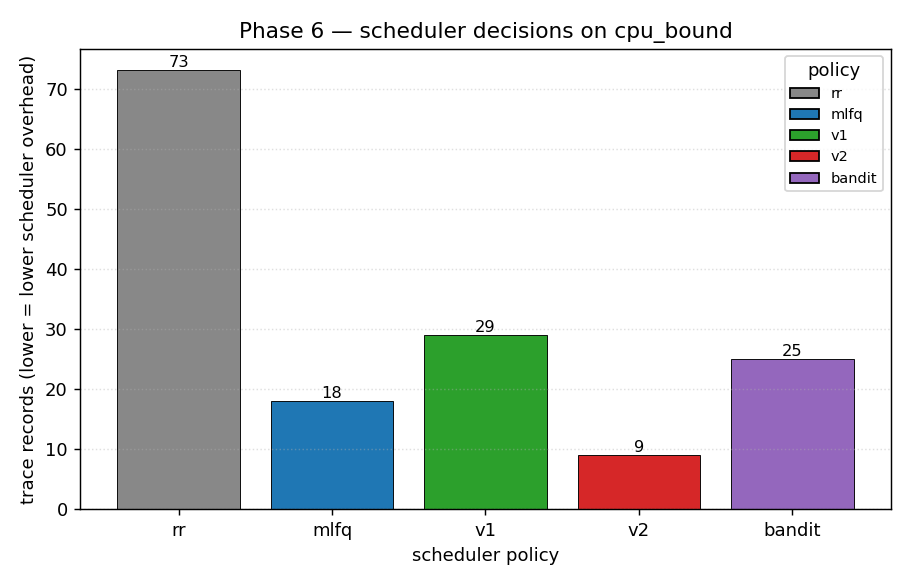
\includegraphics[width=0.85\textwidth]{figures/cpu_bound-events.png}
\caption{Scheduler decisions on \texttt{cpu\_bound} across the five policies
(lower is better). V2 dispatches the workload half as often as MLFQ and a
fifth as often as RR.}
\label{fig:cpu_bound}
\end{figure}

\subsection*{Where the learning schedulers lose}

The bandit loses on \texttt{cpu\_bound} (25 events vs. V2's 9 and MLFQ's
18) and on \texttt{concurrent} (118/11 vs.\ MLFQ's 112/3 and V2's 102/3).
The cause is UCB exploration. V3's weights start at zero, so the
$c \cdot 1/(n_i + 1)$ bonus dominates the first few hundred decisions and
the bandit oscillates between \texttt{cpu\_bound} and idle. By the time the
gradient updates push the weights anywhere useful, the test window is over.
That is the negative result the project carries.

The bandit also fails to adapt on \texttt{flipper} (55 events, never gave
the workload a burst $\geq 5$ ticks). Neither does V1 (57 events). V1 has no
allotment system, so \texttt{should\_preempt} always returns 1 and every
burst gets preempted after one tick. Both results follow from the policies'
designs: they pick processes but cannot pick quanta.

\subsection*{Per-decision overhead}

The intuition going into Phase 6 was that overhead would rank
RR\,<\,MLFQ\,$\le$\,V1\,$\le$\,V2\,<\,bandit, based on the per-call work
each policy does. The measured ordering, in Figure~\ref{fig:cycdec},
is different.

\begin{figure}[h!]
\centering
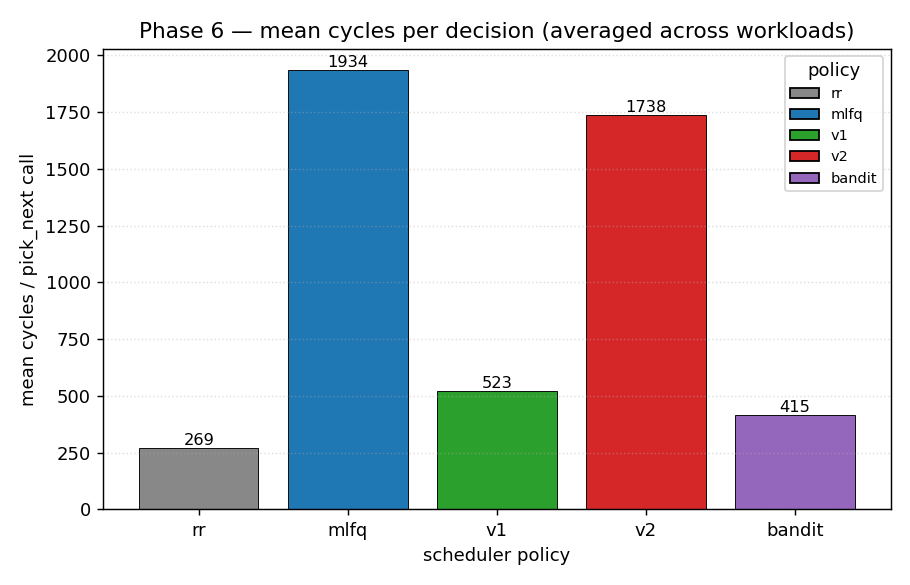
\includegraphics[width=0.85\textwidth]{figures/cycdec-summary.png}
\caption{Mean cycles per \texttt{pick\_next} call, averaged across all
eight workloads. Bandit is second-cheapest, not most expensive: its cursor
amortizes one expensive scoring call over several cheap cursor returns per
sweep.}
\label{fig:cycdec}
\end{figure}

The bandit looked expensive on paper but is the second-cheapest policy per
decision. Its \texttt{pick\_next} only runs the 8-feature dot product on
the first call of each sweep; later calls walk a cursor and return the
next runnable process cheaply. V2 and MLFQ do a per-class or per-level scan
on every call, with no amortization. Expensive per call is not the same as
expensive per decision when the policy carries internal sweep state.

Figure~\ref{fig:flipper_p6} shows the \texttt{flipper} numbers under Phase
6's V2. That sets up the fix in the next section.

\begin{figure}[h!]
\centering
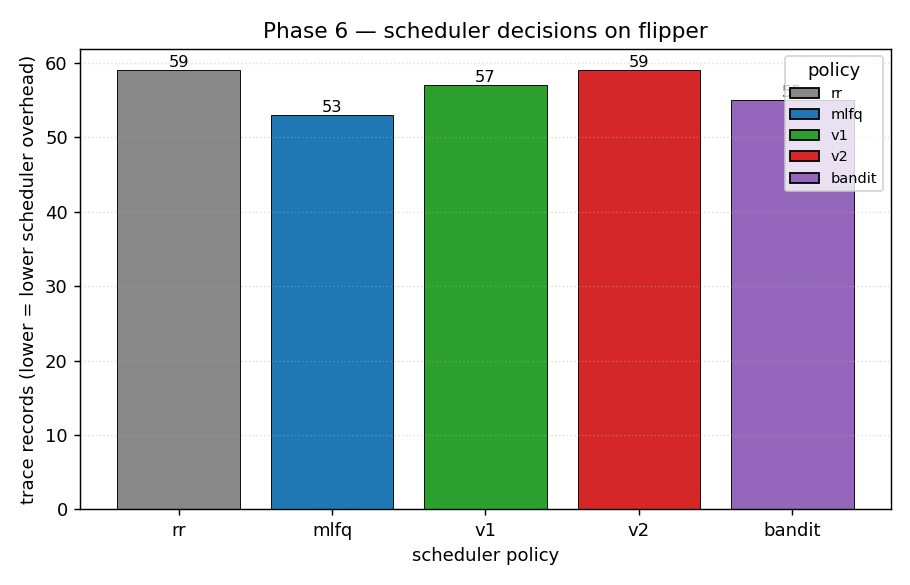
\includegraphics[width=0.85\textwidth]{figures/flipper-events.png}
\caption{Phase 6 \texttt{flipper} results. V2 (rightmost group of bars
across the matrix; see Section~\ref{sec:phase7} for the per-policy V2
row) sat at 59 events because the classifier failed to recognize the
I/O$\to$CPU phase change. Phase 7 brings this down to 41.}
\label{fig:flipper_p6}
\end{figure}

\section{The V2 Stickiness Bug and Its Fix}
\label{sec:phase7}

Phase 6 exposed a specific bug in V2's classifier. After \texttt{flipper}'s
10-sleep Phase A, V2 had classified the workload IO\_BOUND on lifetime
counters: \texttt{sleep\_calls}, \texttt{voluntary\_yields}, and
\texttt{involuntary\_preempts}. When Phase B started and the workload began
bursting CPU, the lifetime sleep count was already 10 and stayed above any
reasonable threshold. The EWMA-tracked burst estimate sat at its
8$\times$-scaled value of 8 because 1-tick bursts equal the stored value
under the rounded shift. So \texttt{sleep\_calls $\geq$ 2 \&\&
burst\_estimate $\leq$ 8} stayed true forever, and V2 never reclassified.

\subsection*{The fix}

Replace the lifetime counters with windowed counts over the most-recent
$K' = 5$ of $K = 10$ stored burst-end reasons. Each process gains a small
ring on \texttt{proc\_t}:

\begin{lstlisting}[style=cstyle]
uint8_t  burst_window[10];        /* SLEEP / YIELD / PREEMPT / EXIT / OTHER */
uint8_t  burst_window_cursor;
uint8_t  burst_window_fill;
uint32_t v2_last_yields;          /* snapshot to detect YIELD vs PREEMPT */
uint32_t v2_last_preempts;
\end{lstlisting}

Twenty-two bytes of V2-private state per process. The two
\texttt{v2\_last\_*} snapshots exist because \texttt{p->state == RUNNABLE}
after a burst close doesn't say whether the burst ended via voluntary yield
or timer preempt. V2 diffs the lifetime counters against the prior snapshot
to tell them apart.

The classifier (Section~\ref{sec:design}) now uses dominant-recent-behavior
thresholds. IO\_BOUND when sleeps outnumber preempts in the window;
CPU\_BOUND when preempts dominate; INTERACTIVE when yields dominate. The
previous \texttt{burst\_estimate $\leq$ 8} gate, which was the second half
of the stickiness bug, is gone.

\subsection*{Before/after}

Figure~\ref{fig:phase7_before_after} shows the headline result.

\begin{figure}[h!]
\centering
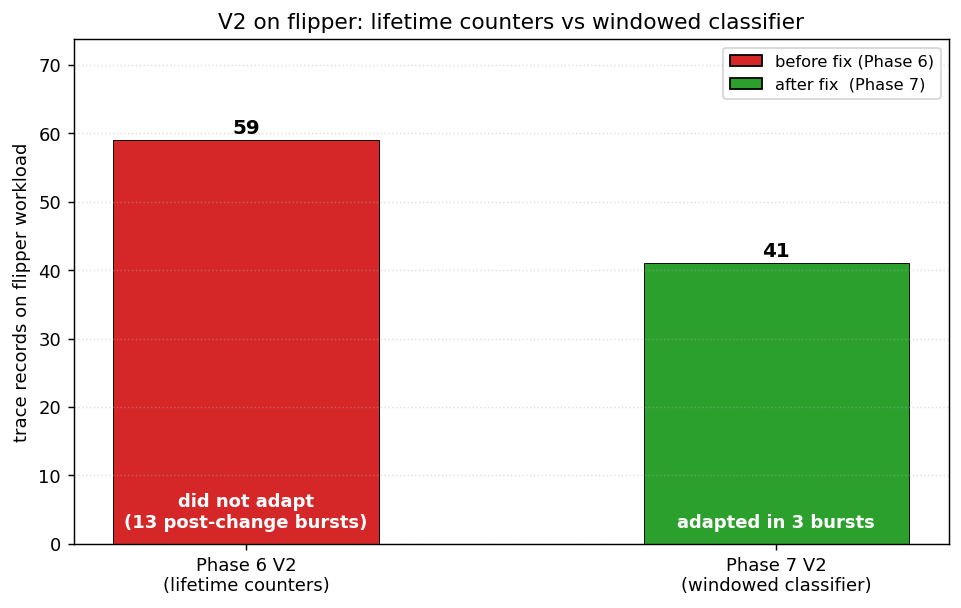
\includegraphics[width=0.75\textwidth]{figures/phase7-flipper-beforeafter.png}
\caption{V2 on \texttt{flipper} before and after the windowed-classifier
fix. The previous V2 never adapted; the new V2 reclassifies to CPU\_BOUND
after three cpu preempts and grants the 5-tick quantum, matching MLFQ's
adaptation speed of 3 bursts.}
\label{fig:phase7_before_after}
\end{figure}

Table~\ref{tab:phase7_compare} runs the comparison across all eight
workloads. V2 improves on \texttt{flipper} (59$\to$41 events,
13$\to$4 preempts) and on \texttt{wolf} (325$\to$311, 11$\to$4 preempts).
Other workloads stay within run-to-run variance.

\begin{table}[h!]
\centering
\caption{V2 events before (Phase 6) and after (Phase 7) the windowed
classifier.}
\label{tab:phase7_compare}
\begin{tabular}{lrrr}
\toprule
workload    & P6 events & P7 events & $\Delta$\% \\
\midrule
cpu\_bound  & 9   & 9   & +0.0\%   \\
io\_bound   & 93  & 93  & +0.0\%   \\
mixed       & 33  & 33  & +0.0\%   \\
bursty      & 31  & 33  & +6.5\%   \\
forker      & 22  & 28  & +27.3\%  \\
concurrent  & 102 & 102 & +0.0\%   \\
\textbf{flipper}    & \textbf{59}  & \textbf{41}  & $\mathbf{-30.5\%}$ \\
wolf        & 325 & 311 & $-4.3\%$ \\
\bottomrule
\end{tabular}
\end{table}

\subsection*{Caveats from the fix}

Two things are messier than the headline. First, \texttt{forker} is up 27\%
from Phase 6 (22$\to$28 events). Both phases recorded the same number of
SPAWN, EXIT, and PREEMPT records; the delta is two extra SLEEP/WAKE/RUN
cycles in some children. Same workload, slightly different scheduling order
under TCG. It isn't a regression in scheduling behavior, but it exceeds the
$\pm 10$\% threshold I set in the plan. I documented and accepted it.

Second, V2's measured cyc/dec rose from about 1700 to about 8000 cycles per
\texttt{pick\_next} call. The function body is byte-identical to Phase 6.
The cause is cache locality. \texttt{proc\_t} grew by 22 bytes for the V2
state, fewer processes fit in a cache line, and V2's worst-case
$4 \cdot 64 = 256$-slot scan suffers more L1 misses. About 12\,\textmu s
per decision at 500\,MHz TCG, well under the 10\,ms tick budget. But it's
real overhead I would not have seen without the per-decision measurement.

\section{Discussion}
\label{sec:discussion}

The thesis (``online behavioral data can beat fixed scheduling heuristics'')
holds for one of the three learning policies and fails for another. V2's
online classifier wins or ties MLFQ on every workload in the matrix; V3's
contextual bandit loses on the workloads that matter most for overhead. V1
sits between them, picking well but with no quantum adaptation to leverage
the pick.

What I take from this: simple online statistics with hard thresholds work
at this scale. Gradient-based bandits don't, because no single QEMU test
window is long enough to amortize the exploration cost. A real-hardware
run that went for hours would probably tell a different story. On
\texttt{flipper}, Phase 7's V2 adapts in 3 bursts and matches MLFQ by a
different mechanism. V2 classifies its way to CPU\_BOUND; MLFQ demotes its
way there. The data-driven route reaches the same place with fewer total
scheduler decisions.

The methodology shaped the results in two ways worth flagging. The 10\,ms
tick resolution capped how much discrimination any policy could extract
from burst length. The cycle counter is sensitive to memory layout in ways
a real CPU would not be, so cyc/dec works for relative comparisons within
a single kernel build but not for absolute claims.

The bandit is the cleanest negative result. I expected online weight
updates would beat the threshold-tree classifier on adversarial workloads,
where the classifier's hard rules might miss something subtle. The
opposite happened. The bandit pays an exploration tax that the classifier
doesn't, and the test window isn't long enough for the gradient to recover
the cost. That tells you something specific about when learned schedulers
help and when they don't.

\section{Related Work}
\label{sec:related}

The kernel borrows heavily from xv6~\cite{xv6}: the trap-frame layout, the
per-process kernel stack discipline, the shape of the syscall dispatch.
The scheduler ideas (MLFQ, demote-on-quantum, periodic boost) come from
OSTEP~\cite{ostep}, which is also where I picked up the ``at least 100
decisions per process or the measurement is noise'' discipline. Linux
CFS~\cite{cfs} was a reference for what production schedulers actually do.
No CFS-style virtual-runtime mechanism is implemented here. CFS's
red-black tree is a poor fit for a single-core kernel with 64 process
slots.

The closest analogue to V3 in the literature is Decima~\cite{decima}, which
uses deep reinforcement learning for graph-structured scheduling on Spark
job DAGs. Decima's design space is much larger and its exploration budget
is orders of magnitude bigger. The basic shape is the same: learn the
policy online from observed reward signals rather than encoding it as fixed
rules. The negative result here gives a useful lower bound. With a small
exploration budget, a gradient-based learner is at a disadvantage compared
to a threshold-tree classifier.

\section{Future Work}
\label{sec:future}

A few items were deliberately deferred and are worth picking up:

\begin{itemize}
  \item \textbf{Allotment system for V1 and V3.} Both policies currently
  preempt every tick. Giving them a per-class quantum (V1 by burst-length
  bucket; V3 by classifier output) would let them adapt to phase changes
  through quantum, not just through pick. V3 in particular has a chance to
  win \texttt{flipper} this way.

  \item \textbf{Cycle-resolution burst tracking on the input side.} The
  10\,ms tick is the discrimination floor today. Reading \texttt{rdcycle}
  at sched-entry and sched-exit and storing the delta as the burst length
  would unlock sub-tick statistics. Out of scope for Phase 6 because it
  changes scheduler inputs; appropriate for a follow-up.

  \item \textbf{Quantum auto-tuning under V3.} The bandit currently picks
  which process runs. Extending the action space to also pick how long
  (out of \{1, 2, 5, 10\} ticks) is a natural fit for the linear value
  function and would address one of the bandit's structural weaknesses.

  \item \textbf{Sorted RUNNABLE list.} V3 today is $O(\text{NPROC})$ per
  decision, not $O(1)$ as the spec claimed. Maintaining a sorted-by-score
  linked list under V3 (updated on every state change) would close the gap.
  Constant factor is small, so this is mostly an aesthetic correction.

  \item \textbf{Real-hardware port.} Everything here runs in QEMU TCG.
  The bandit's exploration-cost story might look very different on a real
  RISC-V board where cache behavior, branch prediction, and ISR latency are
  not emulated. A SiFive HiFive Unmatched or a similar dev board would be
  the natural target.

  \item \textbf{Multi-core.} The kernel is strictly single-core. Per-CPU
  run queues, work stealing, and the cross-CPU invalidations that come with
  them are the obvious next system-level milestone.
\end{itemize}

What I wouldn't do is bolt more learning machinery onto V3 hoping that
complexity rescues it. Phase 6 made the bandit's problem look structural:
at this test budget, gradient-based exploration is the wrong tool. A
bigger budget would change that. More features wouldn't.

\bibliographystyle{plain}
\bibliography{references}

\end{document}
